\section{Main Results}
\label{sec:results}

\subsection{Headline numbers}
\Cref{tab:main} reports the headline accuracy of all five model
configurations on all five benchmarks. \Cref{fig:scores} visualises the
same numbers.

\begin{table}[h]
\centering
\small
\begin{tabular}{lrccccc}
\toprule
\textbf{Model stage} & \textbf{Train size} & \textbf{GSM8K} & \textbf{MATH-500} & \textbf{TheoremQA} & \textbf{HellaSwag} & \textbf{MMLU} \\
\midrule
qwen base         & 0       & 0.0121 & 0.0140 & 0.0576 & 0.5018 & 0.6019 \\
qwen base sft     & 1\,298  & 0.1638 & 0.1440 & 0.1673 & 0.5068 & 0.5993 \\
grpo sampled24k   & 24\,000 & 0.6884 & \textbf{0.4760} & 0.2396 & 0.5101 & \textbf{0.6030} \\
dapo              & 81\,463 & 0.7028 & 0.4180 & 0.2691 & 0.5105 & 0.6014 \\
grpo              & 81\,463 & \textbf{0.7043} & 0.4380 & \textbf{0.2784} & \textbf{0.5112} & 0.5998 \\
\bottomrule
\end{tabular}
\caption{Main result table. Column \emph{Train size} is the number of
training examples actually consumed at the corresponding stage. Best
number per benchmark in \textbf{bold}. The MMLU column is 5-shot accuracy
across 57 subjects; standard error of the MMLU column is approximately
$\pm 0.0039$, so all five MMLU numbers are statistically tied.}
\label{tab:main}
\end{table}

\begin{figure}[h]
\centering
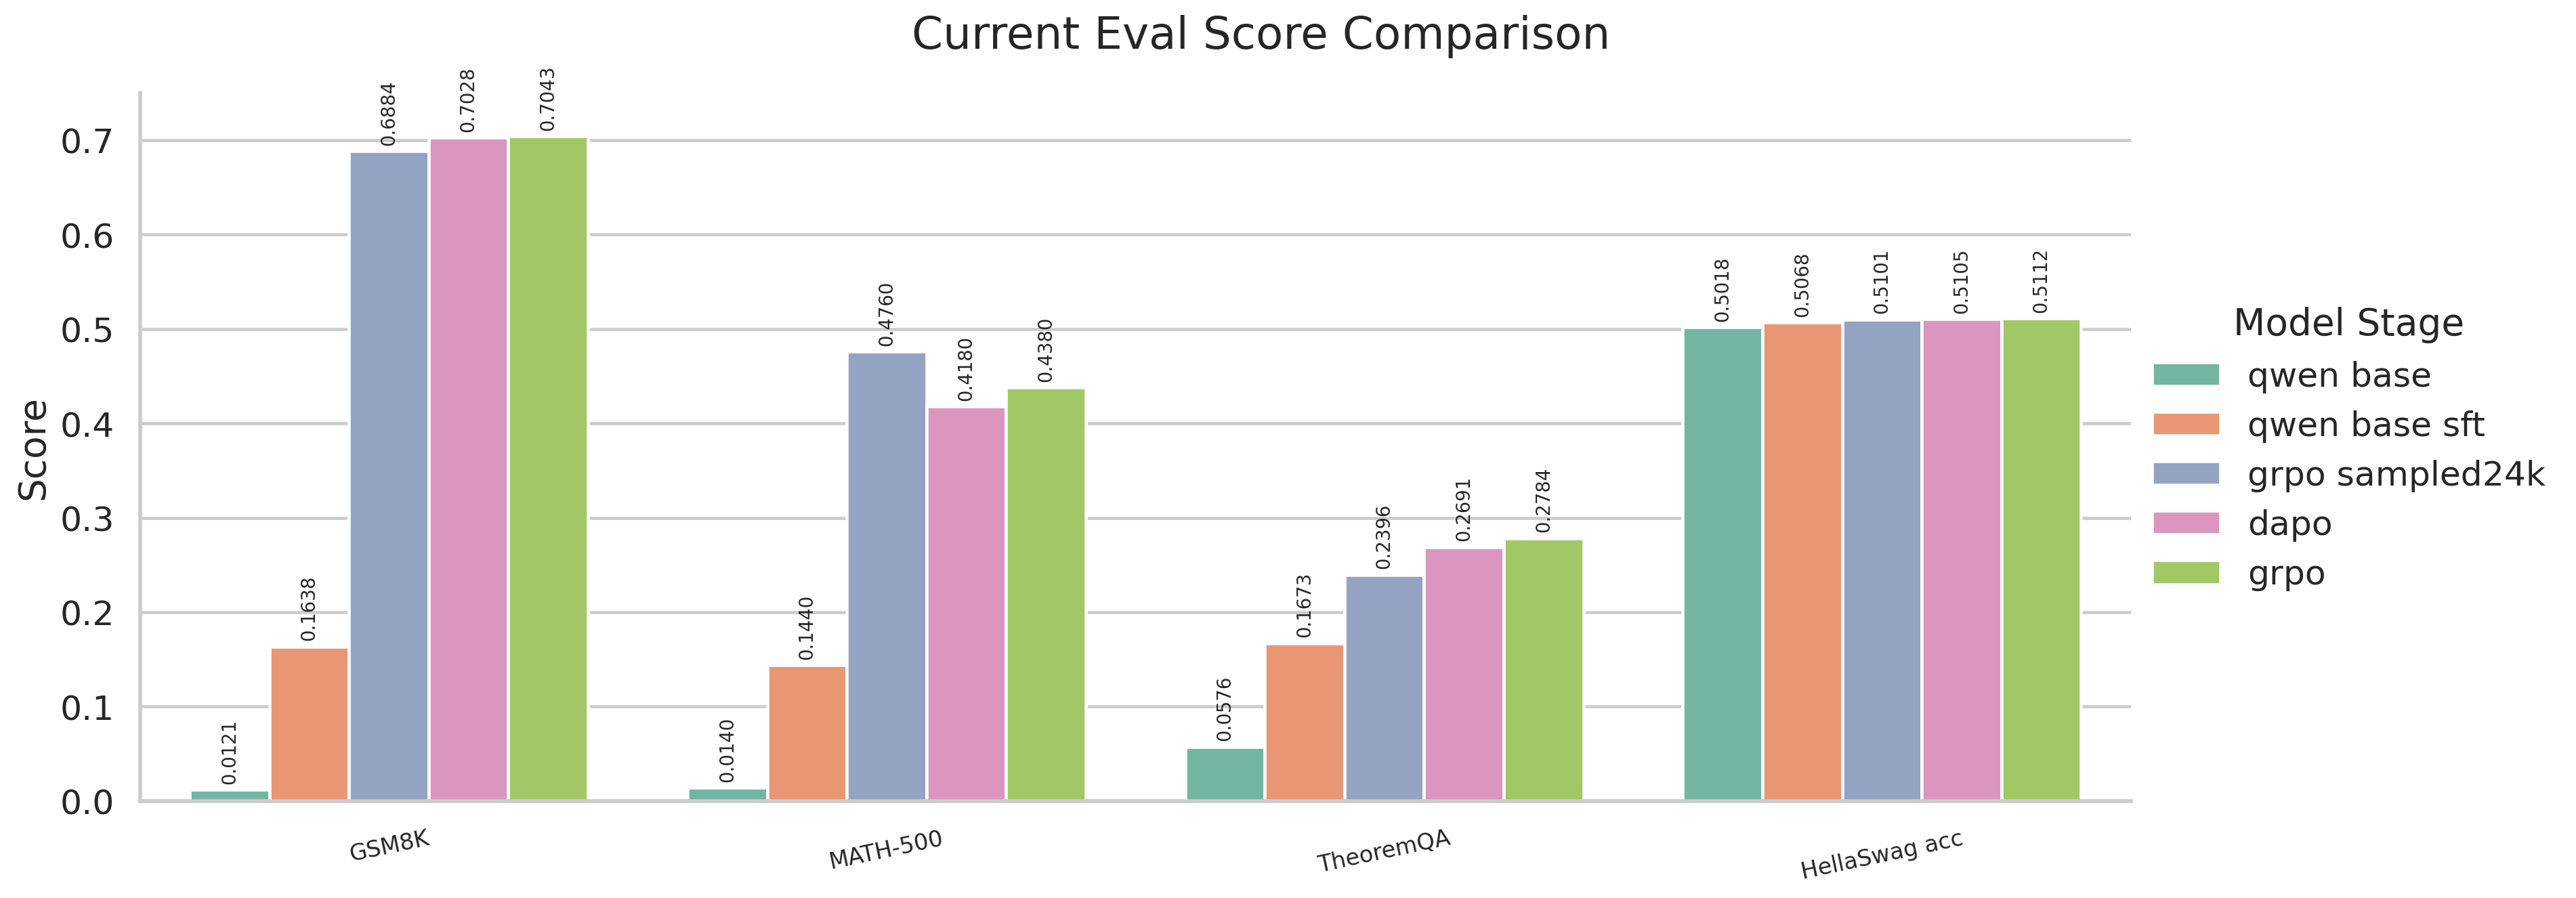
\includegraphics[width=0.92\linewidth]{figures/eval_score_comparison.png}
\caption{Per-benchmark accuracy across the five model stages.}
\label{fig:scores}
\end{figure}

\subsection{Stage-wise reading}
The progression in \cref{tab:main} can be read in three blocks.

\paragraph{Base $\rightarrow$ SFT.}
The base model essentially fails on the math benchmarks under our
instruction template ($\code{GSM8K}=0.012$, $\code{MATH-500}=0.014$,
$\code{TheoremQA}=0.058$), confirming that the failure is one of
\emph{format} rather than \emph{capability}: the base model is not
producing answers in the \code{Final Answer:} format that the
\code{mathrl} extractor recognises. SFT on a small set of 1\,298 cleaned
traces is enough to lift all three math benchmarks by roughly
$10\!\times$ on \code{GSM8K} and \code{MATH-500} and roughly
$3\!\times$ on \code{TheoremQA}.

\paragraph{SFT $\rightarrow$ RL.}
The verifiable-reward RL stage produces a much larger second jump:
\code{GSM8K} climbs from $0.164$ to roughly $0.70$, \code{MATH-500} from
$0.144$ to roughly $0.45$, and \code{TheoremQA} from $0.167$ to roughly
$0.27$. The two RL algorithms (GRPO, DAPO) are nearly tied on
\code{MATH-500} but GRPO is consistently a bit ahead on \code{GSM8K} and
\code{TheoremQA}. The 24K-sampled run sits between SFT and full-pool RL on
\code{GSM8K} and \code{TheoremQA}, but is the strongest on
\code{MATH-500}, suggesting that the difficulty-balanced 24K mixture is
particularly well matched to the harder MATH-500 distribution.

\paragraph{Reward design effects.}
The strong \code{GSM8K} numbers are partly attributable to the
\emph{format} and \emph{cleanliness} terms in \cref{tab:reward-components}:
on saved samples, \code{Final Answer:} coverage stays at 1.0 for both
\code{dapo} and \code{grpo}, with no role-token leakage observed. This
matches the qualitative pattern in \cref{sec:failure}: format errors
disappear after RL and most remaining failures are semantic.

\subsection{Best-per-metric summary}
\begin{itemize}
  \item \code{GSM8K}: \textbf{grpo} ($0.7043$).
  \item \code{MATH-500}: \textbf{grpo sampled24k} ($0.4760$).
  \item \code{TheoremQA}: \textbf{grpo} ($0.2784$).
  \item \code{HellaSwag}: \textbf{grpo} ($0.5112$).
  \item \code{MMLU}: \textbf{grpo sampled24k} ($0.6030$, statistical tie).
\end{itemize}
